\documentclass[convert={density=900,size=1080x800,outext=.png}]{standalone}
\usepackage[utf8]{inputenc}
\usepackage{tikz}

\usetikzlibrary{calc, positioning}
\usetikzlibrary{arrows.meta}
\usetikzlibrary{matrix}
\usetikzlibrary{shadows}
\usepgflibrary{shapes.misc}
\usepgflibrary{{shapes.geometric}}

\pgfdeclarelayer{shadow} 
\pgfsetlayers{shadow,main}
\def\shadowradius{3pt}


\def\mw{2cm}
\def\mh{1.75cm}
\def\trianglecoordinate{2mm}

\newcommand\drawshadowbis[1]{
    \begin{pgfonlayer}{shadow}
        \fill[inner color=black,outer color=white] ($(#1.south west)$) circle (\shadowradius);
        \fill[inner color=black ,outer color=white] ($(#1.north west)$) circle (\shadowradius);
        \fill[inner color=black ,outer color=white] ($(#1.south east)$) circle (\shadowradius);
        \fill[inner color=black,outer color=white] ($(#1.north east)$) circle (\shadowradius);
        \fill[ top color=black, bottom color=white] ($(#1.south west)+((0,-\shadowradius)$) rectangle ($(#1.south east)$);
        \fill[left color=black,right color=white] ($(#1.south east)$) rectangle ($(#1.north east)+((\shadowradius,0)$);
        \fill[bottom color=black,top color=white] ($(#1.north west)$) rectangle ($(#1.north east)+((0,\shadowradius)$);
        \fill[right color=black,left color=white] ($(#1.south west)$) rectangle ($(#1.north west)+(-\shadowradius,0)$);
    \end{pgfonlayer}
    }

\tikzstyle{component} = [draw, fill=white, minimum width=\mw, minimum height=\mh, align=center]

\tikzset{
    border/.style = { 
        draw, rectangle, minimum width=\mw, minimum height=\mh, thick, align=center
    },
    Component/.pic = {
        \node [border, font=\large](-edge){#1}; 
        \draw[thick] ([xshift=\trianglecoordinate] -edge.south) -- ([yshift=\trianglecoordinate] -edge.south);
        \draw[thick] ([xshift=-\trianglecoordinate] -edge.south) -- ([yshift=\trianglecoordinate] -edge.south);
        \draw[thick] (-edge.south) |- ++(-3mm, -4mm) node[xshift=-2mm, yshift=-1mm] {T}; 
    },
}

\tikzset{
    clockborder/.style = { 
        trapezium, trapezium angle=60, minimum width=1cm, draw, very thick
    },
    Clock/.pic = {
        \node [clockborder, shape border rotate=-180](-clockedge){#1};
        \draw[very thick] (-clockedge.east) -- ++(2cm, 0cm);
        \def\sft{0.5}
        \foreach \x in {0, 0.5, 1, 1.5}{
            \draw[very thick] (\x + \sft, 0.1) -| ++(0.25cm, 0.25cm) -| ++ (0.25cm, -0.25cm);
        }
    },
}

\begin{document}
    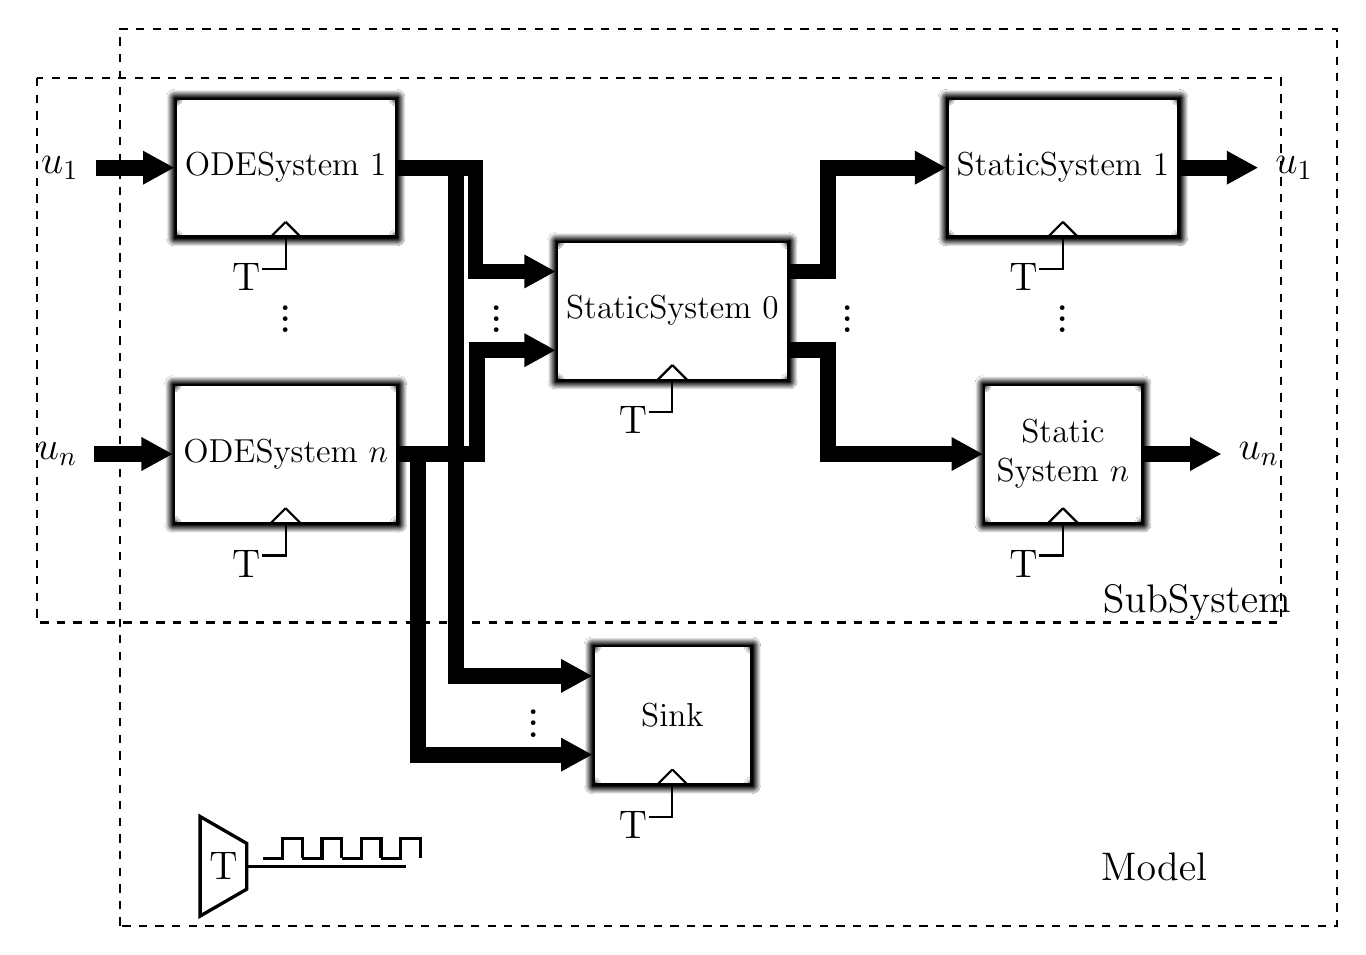
\begin{tikzpicture}[every node/.style={font=\Large}]
        % Place the blocks 
        \matrix (m) [matrix of nodes, ampersand replacement=\&, column sep = 2cm, row sep = -0.75cm, nodes={anchor=center}]{
            \draw pic (ds1) {Component={ODESystem $1$}}; \& \& \draw pic (ss1) {Component={StaticSystem $1$}}; \\
            \draw node[]{\huge $\vdots$}; \& \draw pic (ss0) {Component={StaticSystem $0$}}; \& \draw[ultra thick] node[]{\huge $\vdots$}; \\
            \draw pic (dsn) {Component={ODESystem $n$}}; \& \& \draw pic (ssn) {Component={Static\\System $n$}}; \\[1.5cm]
             \& \draw pic (kutuk) {Component={Sink}}; \& \\
        };
        % Glow the blocks
        \foreach \x in {ds1, dsn, ss0, ss1, ssn, kutuk}{
            \drawshadowbis{\x-edge};
        }
        % Draw connections 
        \begin{scope}[line width=2mm, >={Triangle[width=4mm,length=4mm]}]
            \draw[-] (ds1-edge.east) -- ++(1cm, 0cm) coordinate(a);
            \draw[-] (dsn-edge.east) -- ++(1cm, 0cm) coordinate(b);
            \draw[->] ([yshift=1mm] a) |- ([yshift=0.5cm] ss0-edge.west);
            \draw[->] ([yshift=-1mm] b) |- ([yshift=-0.5cm] ss0-edge.west);
            \draw (ss0-edge.west) node [xshift=-0.75cm]{\huge $\vdots$};
            \draw (ss0-edge.east) node [xshift=0.75cm]{\huge $\vdots$};
            \draw[-] ([yshift=0.5cm] ss0-edge.east) -- ++(0.5cm, 0cm) coordinate(c);
            \draw[-] ([yshift=-0.5cm] ss0-edge.east) -- ++(0.5cm, 0cm) coordinate(d);
            \draw[->] ([yshift=-1mm] c) |- (ss1-edge.west);
            \draw[->] ([yshift=1mm] d) |- (ssn-edge.west);
            \draw[-] (ds1-edge.east) -- ++(0.75cm, 0cm) coordinate(e);
            \draw[-] (dsn-edge.east) -- ++(0.25cm, 0cm) coordinate(f);
            \draw[->] (e) |- ([yshift=0.5cm] kutuk-edge.west);
            \draw[->] (f) |- ([yshift=-0.5cm] kutuk-edge.west);
            \draw (kutuk-edge.west) node [xshift=-0.75cm]{\huge $\vdots$};
            \draw[->] ([xshift=-1cm] ds1-edge.west) node[anchor=east]{$u_1$} -- (ds1-edge.west);
            \draw[->] ([xshift=-1cm] dsn-edge.west) node[anchor=east]{$u_n$} -- (dsn-edge.west);
            \draw[->] (ss1-edge.east) -- ([xshift=1cm] ss1-edge.east) node[anchor=west]{$u_1$};
            \draw[->] (ssn-edge.east) -- ([xshift=1cm] ssn-edge.east) node[anchor=west]{$u_n$};
        \end{scope}

        % Draw rectangle for network
        \draw[thick, dashed] ([xshift=-1.75cm, yshift=0.25cm] ds1-edge.north west) rectangle ([xshift=1.75cm, yshift=-1.25cm] ssn-edge.south east);
        \draw (ssn-edge.south) node[yshift=-1cm, xshift=1.7cm]{SubSystem};

        % \Place clock 
        \begin{scope}[shift={(-5.75cm, -5cm)}]
            \draw pic(clk) {Clock={T}} ;
        \end{scope}

        %  Draw rectangle 
        \draw[dashed, thick] ([xshift=-0.5*\mw, yshift=-0.25*\mh] clk-clockedge.south west) rectangle ([xshift=1*\mw, yshift=0.5*\mh] ss1-edge.north east);
        \draw (clk-clockedge.east) node[yshift=0*\mh, xshift=5.75*\mw]{Model};
    \end{tikzpicture}
\end{document}